\chapter{Introducción}

\textit{Descubrir imágenes hechas píxel de situaciones del día a día,
naturaleza, edificios famosos, personas, y cuantas cosas más, esta es la verdadera esencia de
los nonogramas, también conocidos como hanzies, picross o griddlers.}

\section{Contexto y motivación}

\textit{``No importa lo complejo que sea resolver un nonograma, la clave de
estos rompecabezas reside en que su resolución pueda efectuarse por simple
lógica.''~\cite{dalgety_2017}} Este era el principal propósito de \textit{James Dalgety} y su equipo
de diseñadores, responsables de dar a conocer a occidente este conocido
pasatiempo nipón, impulsado por el arte de la diseñadora \textit{Non Ishida}, más
adelante, responsable de su principal denominación: \textit{"Non"} Ishida y
Dia\textit{"gram"}.

No fue hasta mediados del año 1990, cuando finalmente se dio a conocer los \textit{nonogramas} a escala
mundial, a través de una publicación del periódico británico \textit{The Sunday
Telegraph}. Más adelante, el mismo noticiero adoptó el término bajo el
seudónimo de \textit{griddlers}, publicándolos semanalmente.

A partir de estas publicaciones, se fue difundiendo exponencialmente el famoso puzzle y
se puede encontrar en revistas, otros periódicos y libros. Fue tan notable su
crecimiento que, como otros rompecabezas, alcanzó con prontitud el formato
digital, en forma de sitios web, videojuegos y aplicaciones.

La capacidad creativa que ofrece resulta ilimitada, ya que con tan solo sus
celdas dispuestas en forma de matriz \textit{(filas y columnas)}, permite
representar todo tipo de figuras, siluetas y formas, como si de un lienzo se
tratara. 

Sorprendentemente y a pesar de que nos encontramos en plena era digital, son pocos los
medios que ofrecen una capacidad de creación, más allá del simple
tradicional método del lápiz y papel y así esta herramienta ayuda y otorga al jugador no solo el rol de \textit{resolutor}, sino de \textit{creador},
e impulsa que la cuantía de \textit{nonogramas} a resolver no disminuya.

Un medio digital es ideal para, no solo hacer que esta propiedad de creación sea posible, sino de facilitar su proceso 
y que sea lo más liviano y recreativo posible, de esta forma las aplicaciones móviles, cada vez más conocidas y presentes en nuestra sociedad, constituyen el entorno
perfecto.

Siguiendo esta premisa, lo que sería adecuado es que cualquier usuario pudiera, dentro de lo posible, emplear estos medios
independientemente de cual sean las características técnicas, sistemas operativos y prestaciones de sus dispositivos.

\section{Objetivos}

El presente trabajo explora el mundo de las aplicaciones móviles y propone
una solución software para: i) permitir al usuario resolver \textit{nonogramas} de forma
interactiva ii) dar la oportunidad de crear sus propios puzzles como lo hizo
\textit{James Dalgety} y su equipo y compartirlos con todos los demás usuarios,
promoviendo así una comunidad de entusiastas de este divertido rompecabezas.

Por consiguiente, para el correcto desarrollo y funcionamiento de la aplicación se deben de
cumplir una serie de requerimientos a nivel técnico bien diferenciados:
\begin{itemize}
   \item[$\bullet$] Estudiar y desarrollar una funcionalidad integrada en el aplicativo, con el fin de posibilitar al usuario
   crear y resolver \textit{nonogramas} en un dispositivo móvil, bajo unas variables determinadas, siempre dando prioridad a la experiencia de juego.
   \item[$\bullet$] Implementar un \textit{backend} con el que el aplicativo pueda complementar sus funcionalidades con \textit{servicios en nube},
   tales como la base de datos, sincronización o inicios de sesión.
   \item[$\bullet$] Seguir los principios de \textit{Clean Arquitecture} durante el proceso de desarrollo, implementando patrones de diseño y
   aplicando \textit{suites de test} con el objetivo de aminorar el proceso de mantenimiento.
   \item[$\bullet$] Definir y realizar un MVP \textit{(Mininum Viable Product)}, con el que usuario pueda, en una primera versión,
   hacer uso de sus funciones principales.
\end{itemize}

Finalmente, encontramos requisitos de índole personal, que progresivamente se considerarán como cumplidos durante todo el desarrollo del proyecto,
tales como:

\begin{itemize}
   \item[$\bullet$] Ahondar en el desarrollo de una aplicación móvil, desde su inicio hasta su finalización,
   bebiendo de buenas prácticas y recomendaciones propuestas por artículos, documentaciones y comunidades de desarrolladores.
   \item[$\bullet$] Comprender y profundizar en el extenso mundo de desarrollo de juegos de puzzles, haciendo frente y reduciendo su
   marcada complejidad.
\end{itemize}

\section{Metodología}

El aplicativo resultante, como cualquier otra solución software, debe satisfacer una serie de requerimientos frente un problema
o problemas concretos. %% TODO: Biblio: definición de aplicación
Esta solución podría residir o enfocarse en diferentes plataformas, bajo una perspectiva
tanto de \textit{software} como de \textit{hardware}.

Así mismo, antes de que esté considerada preparada la aplicación para su uso, ha de atravesar por una serie de procesos,
que difieren mucho de un simple desarrollo y en su conjunto reciben el nombre de \textit{System Development Life Cycle (SDLC)},
que corresponden a su ciclo de vida.

\subsection{Ciclo de vida de desarrollo}
Comprender esta serie de procesos, junto a los requisitos recién comentados, es definitorio para elegir una metodología ideal,
que sirva como guía para el correcto desarrollo total del producto.

\begin{itemize}
   \item[$\bullet$] \textbf{Planificación}: identificar los requisitos necesarios para la aplicación,
   considerando y comparando otras soluciones disponibles, para así establecer un \textit{target} o perfil de usuario ideal
   para nuestra aplicación, sin entrar en el apartado técnico.
   \item[$\bullet$] \textbf{Análisis}: establecer los requisitos funcionales de la aplicación, recopilando 
   y anticipándose a aquellos que puedan suponer un problema para la evolución del ciclo de vida.
   \item[$\bullet$] \textbf{Diseño}: documentar las, ya definitivas, características, partes y componentes a integrar en el aplicativo.
   \item[$\bullet$] \textbf{Codificación}: seguir los requisitos ya debidamente documentados e implementarlos creando así el aplicativo. 
   \item[$\bullet$] \textbf{Testing}: realizar \textit{suites de tests} con el fin de encontrar o mostrar
   posibles errores y \textit{bugs}. Además de verificar que los requisitos de la fase de diseño están presentes en la solución.  
   \item[$\bullet$] \textbf{Implantación}: hacer la solución \textit{software} disponible para el usuario, listo
   para su uso.
   \item[$\bullet$] \textbf{Mantenimiento}: monitorizar la experiencia de usuario, contemplando y dando solución a posibles errores,
   además de realizar cambios y mejoras en forma de nuevas versiones.
\end{itemize}

Ya que el desarrollo del producto se ha realizado por una única persona, se optó en una primera instancia, por simplicidad y falta de recursos y equipo por
la \textit{metodología tradicional}: \textit{en cascada}, enfocado en el desarrollo de un único \textit{mínimo producto viable} (MVP).

Sin embargo, esta metodología impediría el uso de prácticas y herramientas propias de las \textit{metodologías ágiles}, como por ejemplo: \textit{la automatización de pruebas} o
\textit{la integración continua}. Por ello, tras un estudio de posibles metodologías del mundo del \textit{software}, finalmente, para el desarrollo del producto, se optaron por las pautas y directrices marcadas por el subrama de la metodología
\textit{Extreme Programming}: \textit{Personal Extreme Programming} (PXP).

\subsection{Metodología Personal Extreme Programming (PXP)} %% http://www.umsl.edu/~hugheyd/is6840/waterfall.html

Esta metodología presenta todos los beneficios que engloba la metodología \textit{Extreme Programming}, normalmente enfocada al \textit{desarrollo ágil para equipos de pequeña envergadura}, con algunas
singularidades que la hacen única.

La idea central de esta subvertiente es la sustitución del concepto \textit{desarrollo por pares}, propia de la metodología \textit{XP}. Este modelo sostiene
que el desarrollo debe de realizarse por dos programadores bajo revisiones continuas por turnos, mientras que en \textit{PXP} la totalidad de las
fases la realiza un solo desarrollador ~\cite{inproceedings}.

\begin{figure}[H]
   \centering
   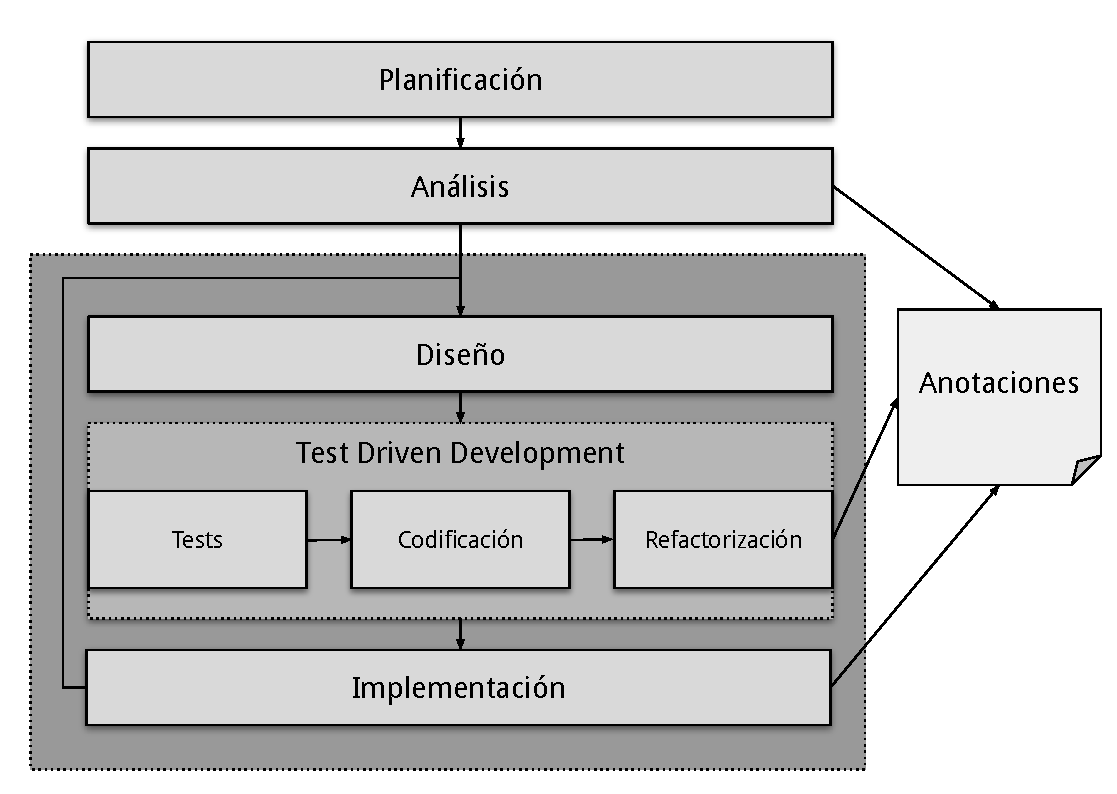
\includegraphics[scale=0.43]{images/pxpdiagram.pdf}
   \caption{Diagrama de la metodología PXP}
   \label{fig:pxpdiagram}
 \end{figure}

 En cuanto al diagrama de flujo de de las diferentes fases que compone
 la metodología \textit{PXP} (\autoref{fig:pxpdiagram}) no difiere mucho del clásico modelo 
 Personal Software Process (\textit{PSP}). Sin embargo, a diferencia de la corriente clásica, este permite realizar iteraciones
 si se requiere algún cambio de diseño en alguno de los requisitos.
 
 Es importante remarcar que al igual que el modelo \textit{PSP}, es recomendable realizar
 durante todo el proceso \textit{anotaciones} de interés como: tiempos reales,
 sugerencias de mejora, detalles..., estas anotaciones serán de gran importancia de cara
 a cambio de requisitos o desarrollo de nuevas funcionalidades.

\begin{itemize}
   \item[$\bullet$] Es necesario hacer hincapié en las etapas tempranas del modelo, ya que son
   las que van a definir de manera correcta los requisitos de la solución. De forma que, si no están bien establecidos, pueden 
   aparecer problemas en el resto de fases~\cite{wiegers2013software}.
   \item[$\bullet$] En la práctica, es recomendable marcar bien los tiempos de cada fase, marcando estimaciones de cada fase y contrastarlas con
   el tiempo real que ha supuesto realizarlas. Esta especie de monitorización se realizará periódicamente y se puede encontrar 
   en el \autoref{chap:A1}
\end{itemize}

\subsection{Enfoque personal}

Pese a que, a nivel personal, por experiencia en entornos profesionales, iba a resultar más cómodo el empleo de la metodología \textit{ágil}, \textit{SCRUM},
existían una serie de razones por las que descartar esta metodología:


\begin{itemize}
   \item[$\bullet$] Para este proyecto, por tratarse de un trabajo individual resultaba insostenible adoptar esta metodología,
   ya que está enfocada a un equipo de desarrollo, mientras que la subvertiente \textit{PXP} enfoca
   la totalidad del desarrollo en un único programador.
   \item[$\bullet$] La metodología \textit{PXP}, junto a su rama padre \textit{XP} promueven el uso de
   tests realizados por el propio programador, para verificar y validar los requisitos, empleando normalmente la metodología \textit{TDD}. Sin embargo, para
   el uso de \textit{SCRUM}, en muchas ocasiones, se requiere de un equipo de \textit{QA} para efectuar la validación de requisitos.
   \item[$\bullet$] En \textit{SCRUM}, los requisitos no pueden ser cambiantes, una vez se definen son definitorios,
   en \textit{PXP} existe un margen de mejora ante un posible problema o estímulo, hecho algo probable en
   escenarios de esta índole.
\end{itemize}



\section{Estructura de la memoria} %%%%% Opcional

El resto de capítulos que conforman la memoria, son los que se resumen a continuación:

\begin{itemize}
   \item[$\bullet$] \textbf{Capítulo 2. Estudio estratégico}: corresponde al conocido apartado \textit{estado del arte}, en el que se realiza una labor 
   de estudio de aquellas soluciones relacionadas con \textit{nonogramas} dentro del mundo digital y que puedan ayudar a la identificación y extracción de requisitos.
   \item[$\bullet$] \textbf{Capítulo 3. Análisis del problema}: en este capítulo se expone la parte de especificación de requisitos,
    identificando aquellos que puedan repercutir negativamente al transcurso del proyecto.
   \item[$\bullet$] \textbf{Capítulo 4. Diseño de la solución}: se muestran las decisiones que se han tomado a nivel de arquitectura, patrones de diseño, 
   y tecnologías empleadas.
   \item[$\bullet$] \textbf{Capítulo 5. Desarrollo de la solución}: se comentan las distintas partes que han compuesto el aplicativo, cómo se comportan y 
   el funcionamiento interno de cada una de ellas, entrando en el apartado técnico.
   \item[$\bullet$] \textbf{Capítulo 6. Pruebas}: se muestran el conjunto de pruebas, que se han desarrollado para la posible identificación de 
   errores y posibles fallos en su ejecución, todas ellas divididas en tipos. 
   \item[$\bullet$] \textbf{Capítulo 7. Implantación y mantenimiento}: se explica el paso que se ha realizado para hacer que el aplicativo sea accesible
   para los usuarios y las medidas para su mantenimiento. 
   \item[$\bullet$] \textbf{Capítulo 8. Manual de uso}: presenta una pequeña demo con el fin de que el usuario se familiarice con el uso de
   la solución, mostrando capturas del mismo.
   \item[$\bullet$] \textbf{Capítulo 9. Conclusión y trabajo Futuro}: contempla las conclusiones que se han obtenido durante la realización del trabajo y
   las mejoras que se tomarán para siguientes versiones del mismo.
   \item[$\bullet$] \textbf{Apéndices}: se muestran anexos relacionados con análisis de tiempos y apartados relacionados con la codificación del
   la solución y análisis de tiempos.
\end{itemize}